\documentclass[12pt,a4paper]{article}
\usepackage[utf8]{inputenc}
\usepackage[spanish]{babel}
\usepackage{graphicx}
\usepackage{hyperref}
\usepackage{geometry}
\geometry{a4paper, margin=2.5cm}
\usepackage{float}

\title{Manual de Usuario - PaTodo}
\author{Equipo de Desarrollo}
\date{\today}

\begin{document}

\maketitle

\section{Introducción}
Bienvenido a \textbf{PaTodo}, la plataforma bajo demanda que te conecta rápidamente con profesionales de confianza para resolver tus necesidades al instante (plomería, jardinería, cambio de llantas, etc.).

\section{Registro e Inicio de Sesión}
Para utilizar PaTodo (ya sea para contratar o para ofrecer servicios), necesitas crear una cuenta.
\begin{enumerate}
    \item Abre la aplicación.
    \item Selecciona \textbf{Registrarse} para crear una nueva cuenta o \textbf{Continuar con Google} para acceso rápido.
    \item Completa tu perfil indicando tus datos y seleccionando el rol con el que deseas operar:
    \begin{itemize}
        \item \textbf{Cliente:} Para publicar trabajos y contratar servicios.
        \item \textbf{Trabajador:} Para recibir ofertas y brindar servicios.
        \item \textbf{Ambos:} Para tener la capacidad de hacer las dos cosas.
    \end{itemize}
\end{enumerate}

\begin{figure}[H]
    \centering
    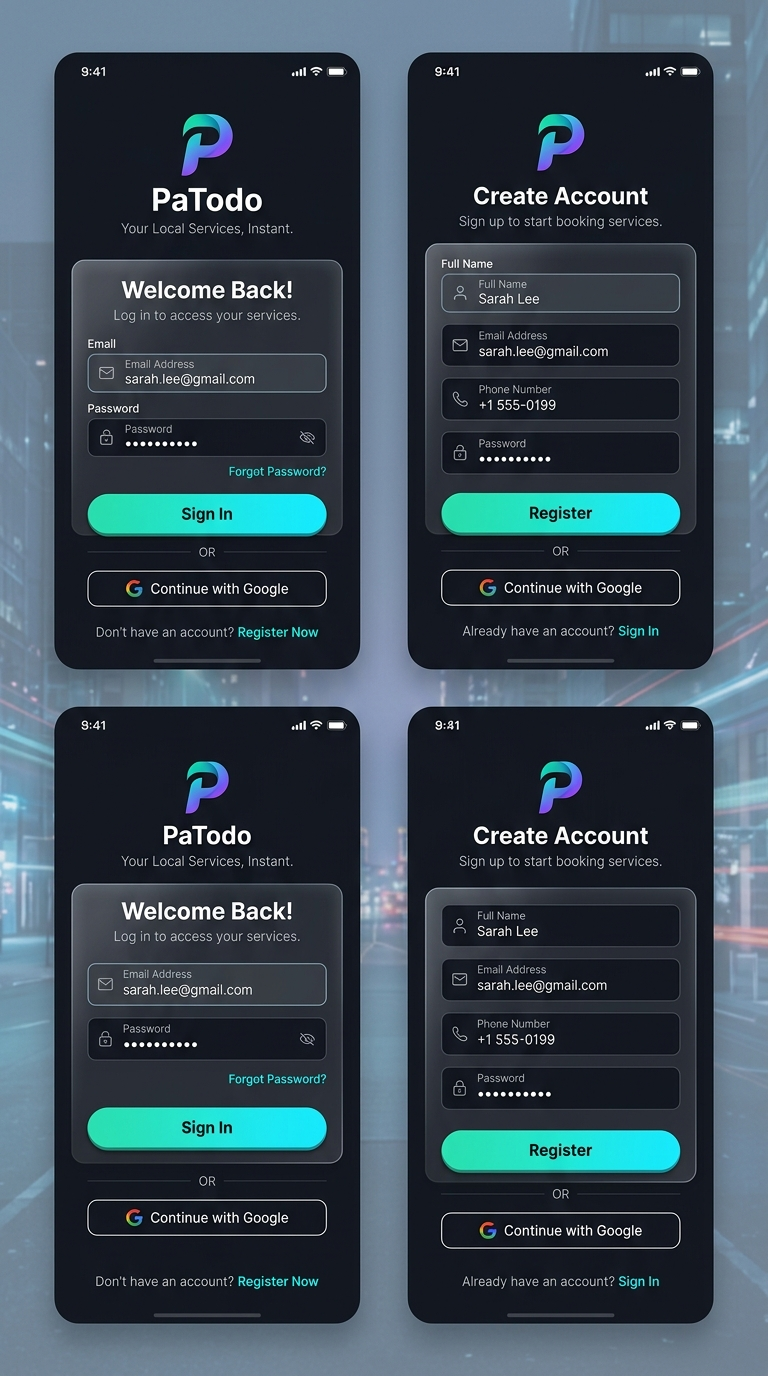
\includegraphics[width=0.45\textwidth]{figuras/login.jpg}
    \caption{Pantalla de Login y Registro}
\end{figure}

\section{Modo Cliente: Publicar Trabajos}
Si necesitas ayuda con un servicio:
\begin{enumerate}
    \item En la pantalla principal \textbf{Inicio}, verás un mapa interactivo mostrando a los trabajadores que se encuentran cerca de ti.
    \item Toca en el botón \textbf{+ Publicar Trabajo} o selecciona rápidamente una de las \textit{Categorías populares} (ej. Fontanería, Jardinería, Mecánica).
    \item Describe el problema, define la ubicación exacta y sugiere el precio que estás dispuesto a pagar.
    \item ¡Listo! Tu solicitud será visible para los profesionales cercanos. Revisa las notificaciones para ver las ofertas que recibas.
\end{enumerate}

\begin{figure}[H]
    \centering
    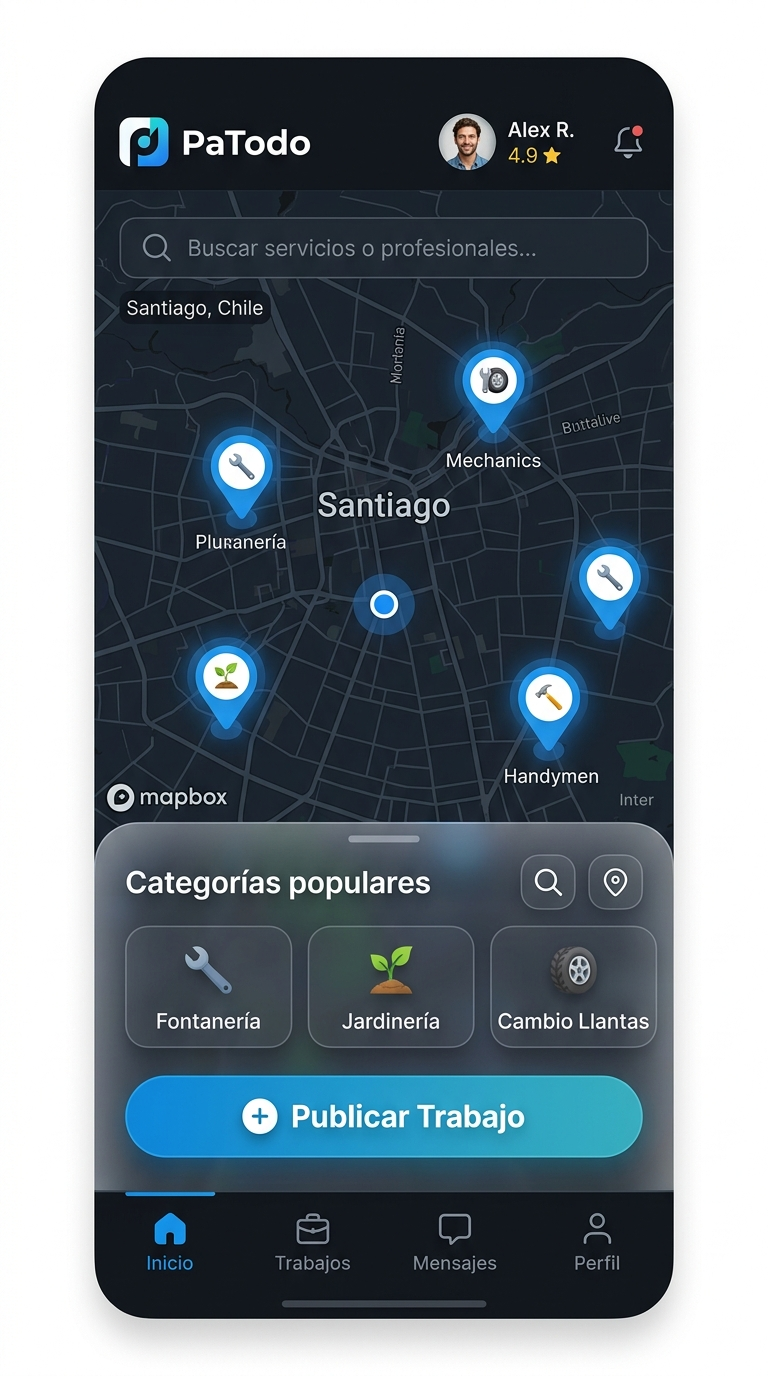
\includegraphics[width=0.45\textwidth]{figuras/client_home.jpg}
    \caption{Pantalla Principal - Vista de Cliente}
\end{figure}

\section{Modo Trabajador: Buscar y Ofertar}
Si eres un profesional ofreciendo tus servicios:
\begin{enumerate}
    \item Dirígete a la pestaña de \textbf{Trabajos} u \textbf{Ofertas}.
    \item Verás una lista actualizada de los trabajos solicitados cerca de tu ubicación. Las tarjetas de trabajo incluyen el título, la distancia, la urgencia y el precio propuesto por el cliente.
    \item Toca en \textbf{Enviar Oferta} en el trabajo que te interese.
    \item Podrás aceptar el precio sugerido o proponer uno distinto, además de indicar el tiempo estimado de llegada al lugar.
\end{enumerate}

\begin{figure}[H]
    \centering
    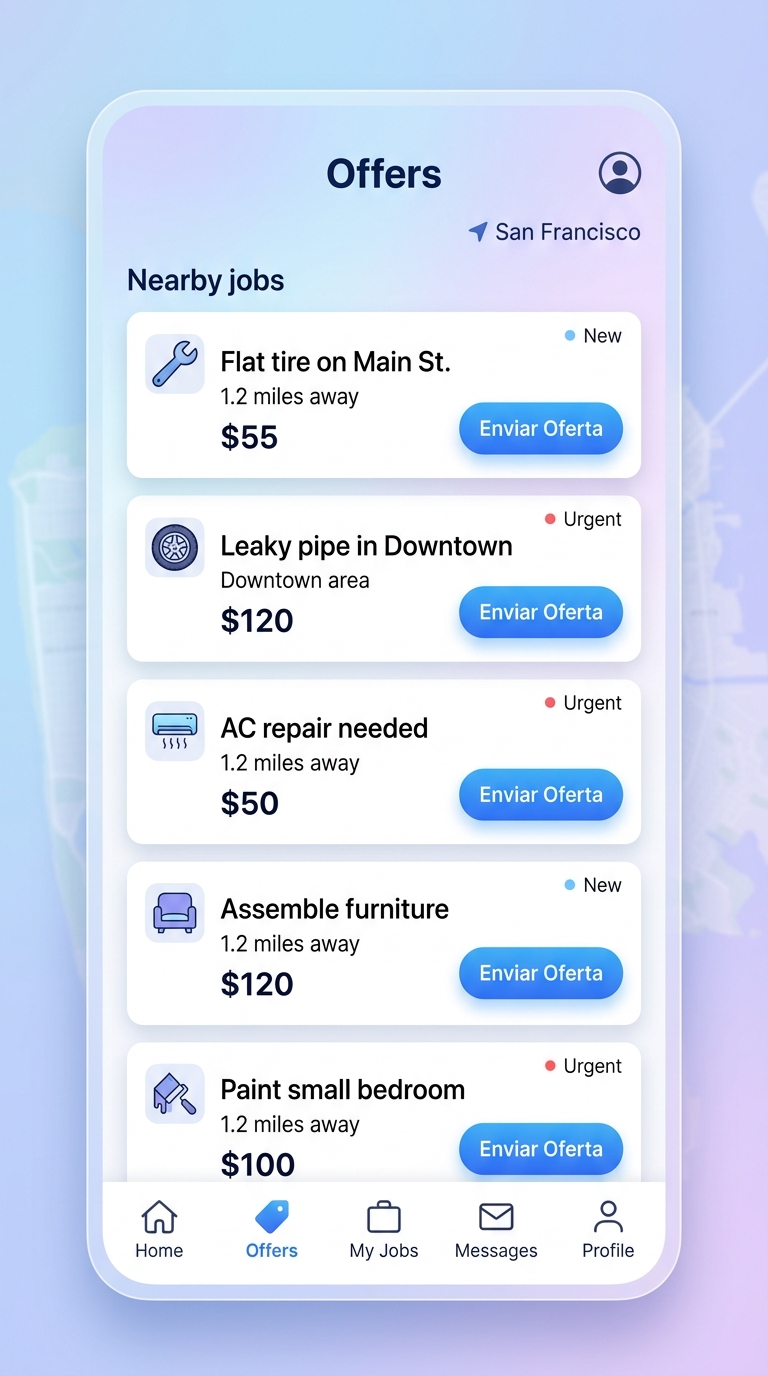
\includegraphics[width=0.45\textwidth]{figuras/worker_offers.jpg}
    \caption{Lista de Ofertas - Vista de Trabajador}
\end{figure}

\section{Comunicación y Finalización}
\begin{itemize}
    \item \textbf{Chat y Llamadas Seguras:} Una vez que el cliente acepta una oferta, se habilitará un chat privado en la pestaña \textbf{Mensajes}. También podrán iniciar llamadas de voz directamente desde la app sin exponer sus números de teléfono personales.
    \item \textbf{Navegación:} La aplicación calculará la ruta óptima para que el trabajador pueda llegar al destino sin problemas.
    \item \textbf{Calificación:} Al terminar el trabajo de forma exitosa, el cliente tendrá la opción de dejar una reseña y calificar el servicio (1 a 5 estrellas). ¡Mantener una buena calificación te ayudará a conseguir más ofertas!
\end{itemize}

\end{document}
